%
% File acl2020.tex
%
%% Based on the style files for ACL 2020, which were
%% Based on the style files for ACL 2018, NAACL 2018/19, which were
%% Based on the style files for ACL-2015, with some improvements
%%  taken from the NAACL-2016 style
%% Based on the style files for ACL-2014, which were, in turn,
%% based on ACL-2013, ACL-2012, ACL-2011, ACL-2010, ACL-IJCNLP-2009,
%% EACL-2009, IJCNLP-2008...
%% Based on the style files for EACL 2006 by 
%%e.agirre@ehu.es or Sergi.Balari@uab.es
%% and that of ACL 08 by Joakim Nivre and Noah Smith

\documentclass[11pt,a4paper]{article}
\usepackage[hyperref]{acl2020}

\usepackage{amsmath}
\usepackage{amsfonts}
\usepackage{amssymb}
\usepackage{booktabs}
\usepackage{color, colortbl}
\usepackage{enumitem}
\usepackage{graphicx}
\usepackage{hyperref}
\usepackage[latin1]{inputenc}
\usepackage{latexsym}
\usepackage{multirow}
\usepackage{times}
\usepackage{url}
\usepackage{xcolor}
\usepackage{xspace}

\renewcommand{\UrlFont}{\ttfamily\small}

%\usepackage{microtype}

%\aclfinalcopy % Uncomment this line for the final submission
%\def\aclpaperid{***} %  Enter the acl Paper ID here

%\setlength\titlebox{5cm}
% You can expand the titlebox if you need extra space
% to show all the authors. Please do not make the titlebox
% smaller than 5cm (the original size); we will check this
% in the camera-ready version and ask you to change it back.

\newcommand{\sz}[1]{\textcolor{blue}{\emph{//sz: #1//}}}
\newcommand{\gbt}[1]{\textcolor{orange}{\emph{//gbt: #1//}}}
\newcommand{\cs}[1]{\textcolor{green!60!black}{\emph{//cs: #1//}}}
\newcommand{\mw}[1]{\textcolor{orange!60!black}{\emph{//mw: #1//}}}

% To streamline frequently used terms:
\newcommand{\langvis}{language\ \&\ vision\xspace}
\newcommand{\lv}{L\&V\xspace}
\newcommand{\mn}{ManyNames\xspace}
\newcommand{\vg}{VisualGenome\xspace}

\newcommand{\cat}[1]{\textsc{#1}}
\newcommand{\name}[1]{\textsl{#1}}

% Terms that need to be replaced throughout the paper by more appropriate ones:
\newcommand{\arbitrary}{arbitrary$\rightarrow$?\xspace}


\title{Supplementary Material}

\author{First Author \\
	Affiliation / Address line 1 \\
	Affiliation / Address line 2 \\
	Affiliation / Address line 3 \\
	\texttt{email@domain} \\\And
	Second Author \\
	Affiliation / Address line 1 \\
	Affiliation / Address line 2 \\
	Affiliation / Address line 3 \\
	\texttt{email@domain} \\}

\date{}

\begin{document}


\section{Verification Procedure with AMT}
\label{sec:verif}
As summarized in the main paper, we recruited annotators from Amazon Mechanical Turk\footnote{
	\url{https://mturk.com}
} (AMT) to categorize the object-name pairs from the \mn dataset.
Here we detail the task interface, our population of annotators, the quality control measures we took, and the approval/rejection policy and rewards.
Basic numbers and results are summarized in Table~\ref{tab:verification-numbers}.

\paragraph{Task interface and Instructions}
The task interface is shown in Figure~\ref{fig:verification-interface}.
We provided (and clarified by means of explanation and visual examples, not show in the image) the following definition: \textit{a name is ``adequate'' if there is an object in the image, whose visible parts are tightly circumscribed by the red bounding box, that one could reasonably call by that name}.
The buttons in the interface all contained suitable pictorial representations to facilitate learning the task.
We provided detailed instructions and examples at the top, as well as informative hover texts on all the buttons and some of the highlighted terms in the task headings.
The hover text of the coloring/clustering task contained a visual example of a completed color grid.
Feedback from annotators suggested that the task interface was intuitive, and they generally enjoyed doing our tasks.
\begin{figure*}[t]
	\centering
	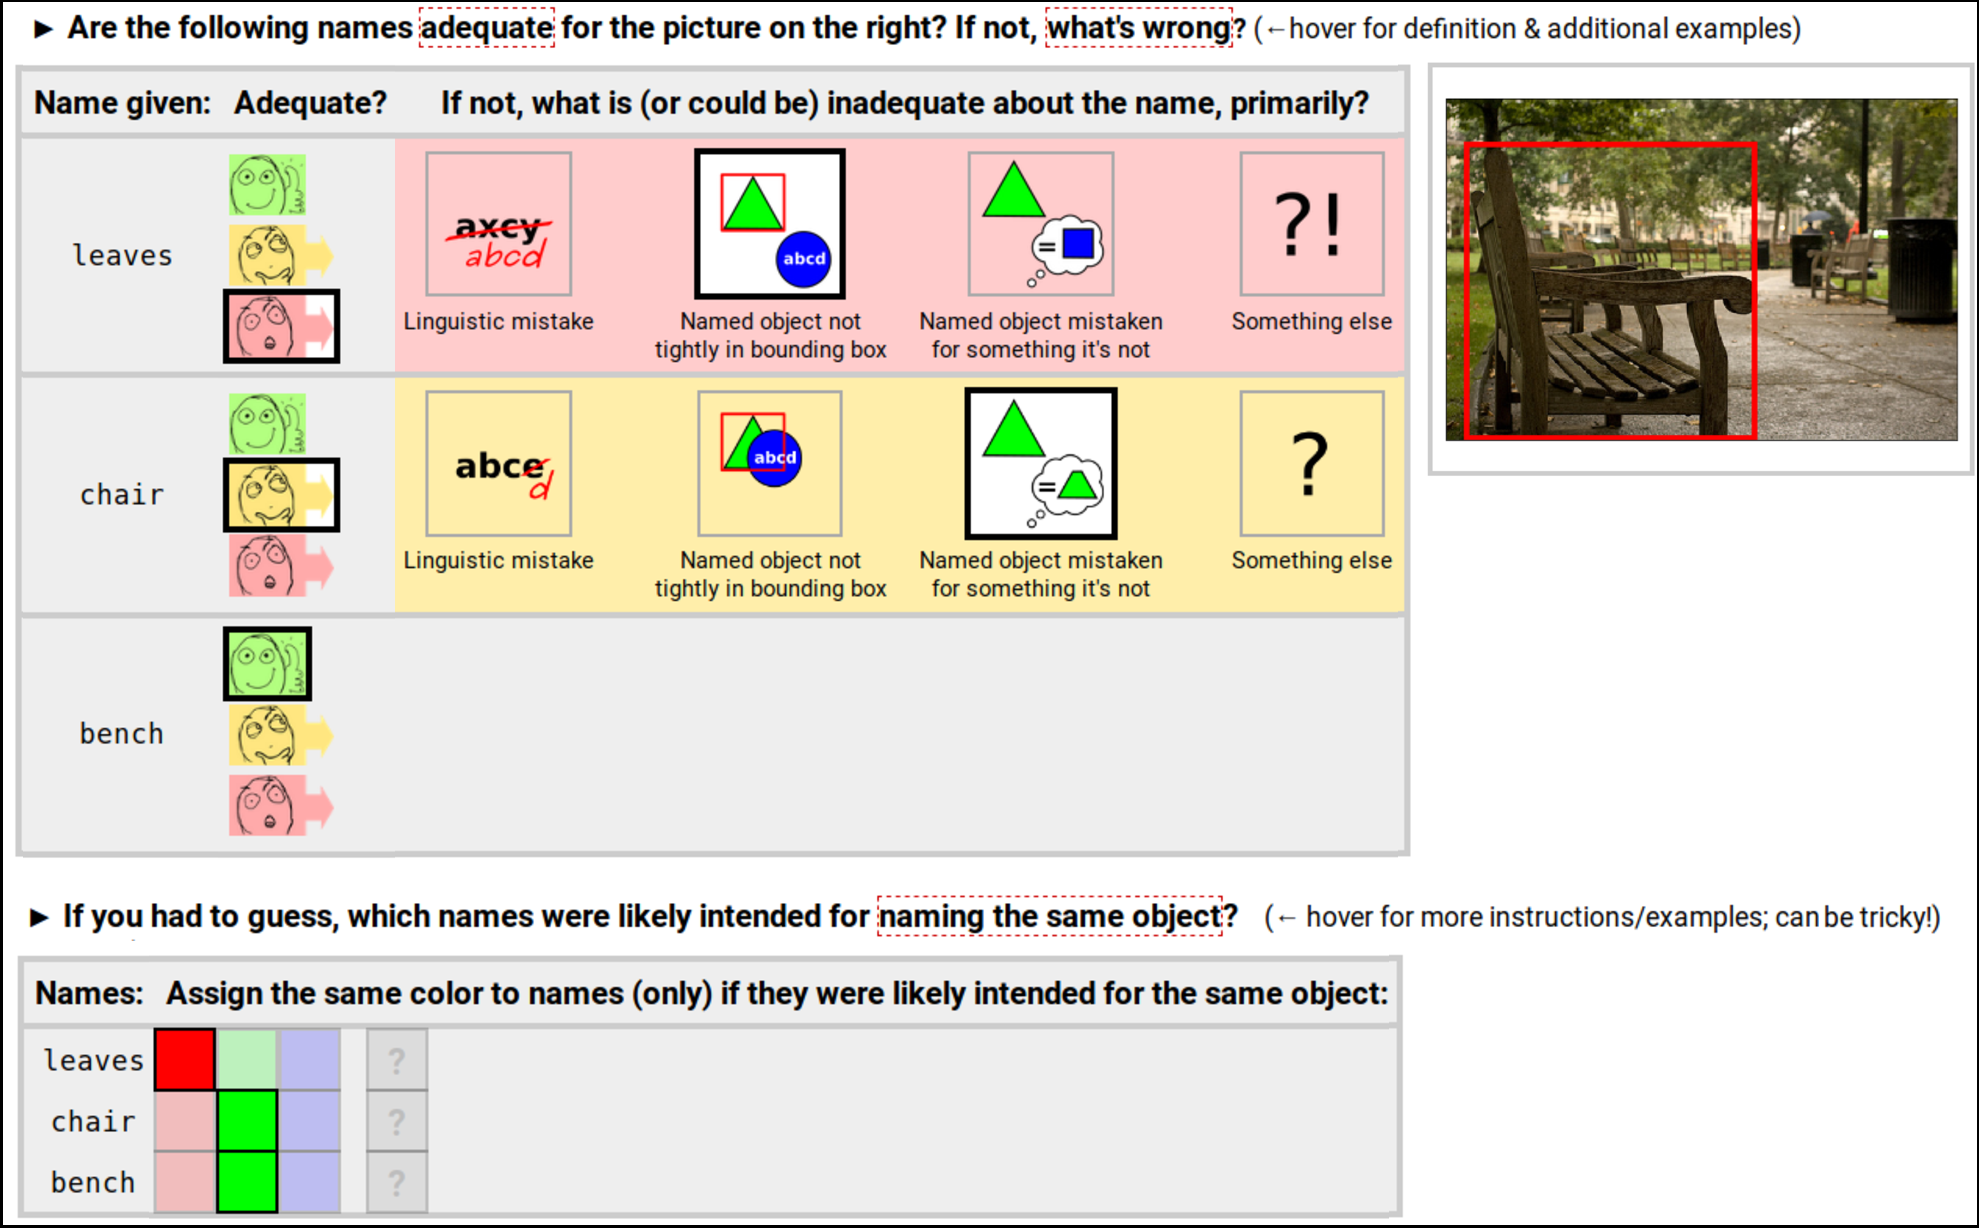
\includegraphics[width=\textwidth]{images/verification-interface.pdf}
	\caption{A screenshot of our verification task interface. Up to ten names could be shown for an image in this way (the number of available colors in the second task would increase accordingly).}
	\label{fig:verification-interface}
\end{figure*}


\paragraph{Annotators}
We used AMT's system of qualifications to set the following entry requirements: at least 1000 tasks completed with over 98\% approval rate, and physical location in country with English as a common language (UK, Ireland, USA, New Zealand, Australia), as a proxy for linguistic background.
We published our tasks in eight batches of a few hundred each, with one or two days in between batches.
In every batch we set a limit, using the UniqueTurker script\footnote{\url{https://uniqueturker.myleott.com/}}, to 50 tasks per annotator, which ensured a diversity of annotators (hence more informative inter-annotator agreement scores), enabled us to accumulate a larger crowd of typically recurring annotators -- ultimately 255 annotators in total -- and prevented unreliable annotators from doing too many of our tasks before we had the ability to block them (based on our quality control, see below) by assigning a blocking qualification to them, which we did in between batches.
\begin{table}[t]
	\centering
	\small
	\begin{tabular}{|ll|ll|}
		\hline
		\multicolumn{2}{|c|}{\textbf{Task setup:}} & \multicolumn{2}{c|}{\textbf{Results:}} \\ \hline
		Images: & 19,427 &
		Annotators: & 255 \\
		Img-name pairs: & 69,356 &
		Annotators/task: & $\geq$ 3 \\
		Tasks: & 3,052 &
		Adeq. mean: & \hspace{-3em}.80 (std .093)\\
		Images/task: & 6-7 &			
		Agreement (adeq.) & 88\% \\ 
		Names/task: & 20-30 &
		Agr. (inadeq. type): & 86\% \\
		\multicolumn{2}{|l|}{Task reward: \ \$.50 (+.15)} & 
		Agr. (same-obj): & 94\% \\
		\hline
	\end{tabular}
	\caption{Verification task overview. 
		\label{tab:verification-numbers}}
\end{table}



\paragraph{Quality Control}
Every task (comprising 20-30 names) contained around 15\% automatically generated quality control items of various kinds, based on several simple automatic rules that are \emph{mostly} true:
\begin{itemize}
	\item If the \mn entry-level name is equivalent to the original \vg name, assume it is an adequate name.
	\item Duplicate one of the \mn names for the object (with a strong bias for selecting the entry-level name), randomly insert a plausible-looking typo, assume it counts as a ``linguistic error''.
	\item Insert a \vg name for a different object in the same image, with a sufficiently different bounding box, and assume it is a ``bounding box error''.
	\item Insert a random \mn name from the full vocabulary of \mn names, that is not among the \mn names for the present image, and assume this will qualify as an ''other error''.
	\item Take any two names among the \mn-names for the object that are synonyms according to WordNet, and assume that they should get the same adequacy rating and inadequacy type.
\end{itemize}
Moreover, we checked for consistency between the adequacy/inadequacy type categorization task and the subsequent coloring/clustering task in various ways, e.g., if one name is judged adequate and the other a ``bounding box error'', then they should be assigned different colors.
None of these rules were exceptionless, but put together they gave a pretty clear picture.
After ignoring the quality controls that no annotator did in the way intended (assuming those must be exceptions to our rules), about half of our tasks scored a 100\% accurate on the quality controls.
We would award those annotators a bonus (see below).
We used our quality control items for providing direct feedback to our annotators: when trying to submit their results, participants would get a warning if their accuracy on the quality control items was below 90\%, and the advice to stop doing these tasks if it was below 80\%, with the option to double-check their responses.
This was meant to encourage them to pay attention, and to discourage them from doing too many of our tasks if they would continue to get warnings.
We did not prevent them from submitting however, and we made sure they understood that getting the warning would not mean automatic rejection.

\paragraph{Approval/Rejection, Compensation and Bonus}
Upon task approval, annotators were awarded \$0.50.
Annotators who scored 100\% accuracy on our quality controls (ignoring ones that no annotator did correctly) received a bonus of \$0.15, as we announced in the instructions for extra incentive.
After every round we blocked annotators with average accuracy below 90\%, removed their results from the dataset and republished the relevant tasks to ensure consistent coverage of the \mn data.
Approval/rejection was decided on a much lower threshold of 70\% accuracy, and with various mechanisms in place for more leniency, e.g., the first task below this threshold would be approved nonetheless; and any task below this threshold would be approved if the annotator's average accuracy was above 90\%.
We rejected less than 2\% of the tasks.



%\bibliographystyle{acl_natbib}
%\bibliography{naming}
\end{document}